\documentclass[Rapport/Rapport_main.tex]{subfiles}
\begin{document}
\section{Integrationstest}\label{sec:rap_integrationstest}
I de følgende afsnit er integrationstestene mellem systemerne kort beskrevet. For en mere detaljeret dokumentation henvises til bilaget "Integrationstest". 

\subsection{Udførsel af integrationstests}
Integrationstestfasen blev udført med en bottom-up tilgang til de forskellige systemer, moduler og komponenter. Her specificerede vi hovedelementer i delsystemerne, som skulle testes og verificeres - når et delsystem blev bekræftet operationel, blev det testet med andre undersystemer indtil alle enheder var integreret i et top-niveau system. \\
Da et delsystem bliver testet isoleret og der laves lokale optimeringer, kan det resulterer i at der opstår uventet fejl, når det sættes sammen i et top-niveau system. Figur \ref{fig:Bottom-Up} viser den hierarkiske rækkefølge af integrationstest. 
\begin{figure}[H]
    \centering
    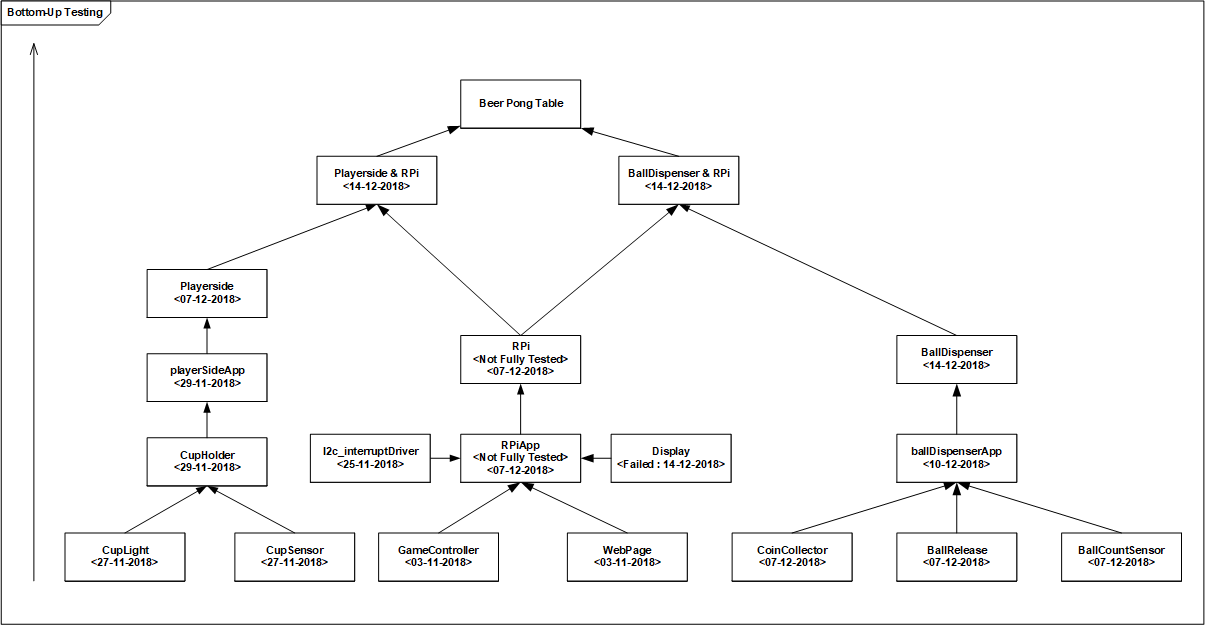
\includegraphics[width=1\textwidth]{Rapport/Test/graphics/Buttom-Up.png}
    \caption{Bottom-up Testing - Her vises den hierarkiske tilgang til integrationstest. Her blev de individuelle moduler integreret i undersystemer først, indtil det til sidst blev sat sammen til et top niveau system. Datoen indikerer hvornår modulet er blevet integreret i det system som pilen peger på - fx GameController og WebPage blev intregeret i RPiApp d. 03 November 2018}
   \label{fig:Bottom-Up}
\end{figure}

\subsubsection{Centrale elementer fra integrationstest}
I dette afsnit redegøres for de centrale elementer i de udførte integrationstest mellem delsystemerne. \\\\
\textbf{Playerside og RPi - GameProgression} \\
Playerside var fuldt integreret, men RPiApp manglede stadig at implementere og integrere Display-klassen. \\
I2C kommunikationen blev tilsluttet mellem Playerside PSoC enheden og RPi'en, samt Analog Discovery til at måle i2c kommunikation (Bits sendt mv.). \\
Kommunkationen var en succes, men der opstod enkelte problemer med flere adgange til I2C bussen. Dette blev fikset ved at tilføje en 'wait\_interruptable' proces, når en enhed tilgår bussen. \\\\
\textbf{Interrupts - Playerside}\\
En af overvejelserne der var før og under integrationstesten for player side, både HW og SW, var at de forskellige delsystemer alle brugte interrupts og de dermed kunne påvirke hinanden negativt når de integreres. Dette viste sig også at være tilfældet. Det blev løst ved at ændre på prioriteten af interrupts. De interrupts der tager kortest tid og er mest kritiske for at systemet virker har en høj prioritet og andre har lavere. Derfor prioriteres interrupts ascocieret med I2C højest og interrupts ascocieret med at blinke lys lavest. Interrupts for Cup Light indstilles til have højere prioritet end for Cup Sensor, da disse interrupts er meget kortere end dem for Cup Sensor \\\\
\textbf{Integrationstest for hele systemet - Beer Pong Table}\\
Efter hele systemet blev sat sammen (Bortset fra Displayet), opstod der flere problemer:
\begin{itemize}
    \item Af ukendelig årsag måtte en computer tilkobles direkte til PSoC-enheden tilsluttet til \textit{Playerside} - ellers virkede det ikke. 
    \item SCL-linjen forblev lav indtil PSoC enhederne blev genstartet - der kunne hermed ikke sendes fra RPi til Playerside
    \item RPi'en læste enten rent højt eller lavt fra PSoC enhederne ved tilfældige tidspunkter, uden nogen konsekvent sammenhæng. 
\end{itemize}
\end{document}